El algoritmo de Berkeley es una técnica de sincronización de reloj utilizada en
sistemas distribuidos. El algoritmo asume que cada nodo de la máquina en la red
no tiene una fuente de tiempo precisa o no posee un servidor UTC.\@

En la \textbf{Clase Master} se elige un nodo individual como nodo maestro de un
grupo de nodos en la red. Este nodo es el nodo principal de la red que actúa
como maestro y el resto de los nodos actúan como esclavos. El nodo maestro se
elige mediante un proceso de elección/algoritmo de elección de líder.

En la \textbf{Clase Slave} los slaves se inicializan y se les asigna el tiempo
en que fueron inicializados, ese tiempo se los asigna la clase master utilizando
la biblioteca \mintinline{shell}{zmq}.
Se utiliza \textbf{localhost}\footnote{Nombre predeterminado que se usa para establecer
  una conexión con la computadora local computadora usando la red de dirección
  de bucle invertido. $127.0.0.1$} y los puetos $1000$, $1001$, $1002$ y $1004$.
No olvidemos que Master es otro Slave, solo que ese Slave se elije como Master.

\begin{figure}[H]
  \centering
  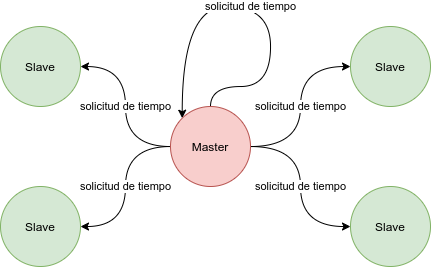
\includegraphics[width=10cm]{1}
  \caption{Solicitud de tiempo para cada Slave y el mismo Master}\label{fig:1}
\end{figure}

Después de la sincronización, cada proceso imprime su reloj lógico para
verificar el resultado de la sincronización.

El Slave maestro calcula la diferencia de tiempo promedio entre todas las horas
de reloj recibidas y la hora de reloj proporcionada por el reloj del sistema
maestro. Esta diferencia de tiempo promedio se agrega a la hora actual en el
reloj del sistema principal y se transmite a través de la red.

\begin{figure}[H]
  \centering
  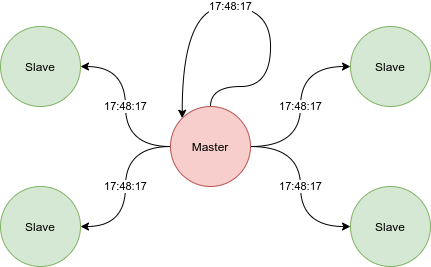
\includegraphics[width=10cm]{2}
  \caption{Sincronización del tiempo}\label{fig:2}
\end{figure}

\begin{figure}[H]
  \centering
  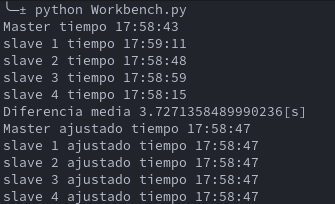
\includegraphics[width=10cm]{3}
  \caption{Ejecución de \mintinline{shell}{Workbrench.py}}\label{fig:3}
\end{figure}


% \begin{minted}[
%   frame=lines,
%   framesep=2mm,
%   baselinestretch=1.2,
%   bgcolor=LightGray,
%   fontsize=\footnotesize,
%   linenos
%   ]{python}
% from time import time, gmtime, strftime
% import zmq

% class Master():

%     def __init__(self):
%         self.suma_diferencias = 0
%         self.slaves = []
%         self.tiempos = []
%         self.tiempo_sincronizado = time()
%         self.diferencia_media = 0

%     def registrar_slave(self, port):
%         self.slaves.append(port)

%     def get_time(self):
%         return self.tiempo_sincronizado

%     def get_human_time(self):
%         return strftime("%H:%M:%S",gmtime(self.get_time()))

%     def obtener_tiempos(self):
%         self.tiempos = []
%         for slave in self.slaves:
%             self.tiempos.append(self.obtener_tiempo_slave(slave))

%     def obtener_tiempo_slave(self, slave):
%         context = zmq.Context()
%         socket = context.socket(zmq.REQ)
%         socket.connect("tcp://localhost:{}".format(slave))
%         socket.send("dame_tiempo".encode('utf-8'))
%         return float(socket.recv().decode('utf-8'))

%     def enviar_ajuste(self):
%         cont = 0
%         for slave in self.slaves:
%             dif =  self.tiempo_sincronizado - self.tiempos[cont]
%             context = zmq.Context()
%             socket = context.socket(zmq.REQ)
%             socket.connect("tcp://localhost:{}".format(slave))
%             socket.send(str(dif).encode('utf-8'))
%             cont += 1

%     def work(self):
%         self.obtener_tiempos()
%         self.sumar_diferencias()
%         self.calcular_diferencia_media()
%         self.tiempo_sincronizado = time() + self.diferencia_media
%         self.enviar_ajuste()

%     def calcular_diferencia_media(self):
%         self.diferencia_media = self.suma_diferencias / (len(self.slaves) + 1)

%     def sumar_diferencias(self):
%         self.suma_diferencias = 0
%         for tiempo in self.tiempos:
%             diferencia = tiempo - time()
%             self.suma_diferencias += diferencia
% \end{minted}
